%
% حق نشر 1390-1402 دانش پژوهان ققنوس
% حقوق این اثر محفوظ است.
% 
% استفاده مجدد از متن و یا نتایج این اثر در هر شکل غیر قانونی است مگر اینکه متن حق
% نشر بالا در ابتدای تمامی مستندهای و یا برنامه‌های به دست آمده از این اثر
% بازنویسی شود. این کار باید برای تمامی مستندها، متنهای تبلیغاتی برنامه‌های
% کاربردی و سایر مواردی که از این اثر به دست می‌آید مندرج شده و در قسمت تقدیر از
% صاحب این اثر نام برده شود.
% 
% نام گروه دانش پژوهان ققنوس ممکن است در محصولات دست آمده شده از این اثر درج
% نشود که در این حالت با مطالبی که در بالا اورده شده در تضاد نیست. برای اطلاع
% بیشتر در مورد حق نشر آدرس زیر مراجعه کنید:
% 
% http://dpq.co.ir/licence
%
\section{برگه‌های دیگر}
  علاوه بر برگه نخست برگه‌های دیگری نیز در مستند وجود دارند که جنبه‌های متفاوتی
  از سیستم را مورد بررسی قرار می‌دهند. نصب و راه اندازی، مبانی مورد استفاده در
  سیستم، به کارگیری و خطاهای متداول سیستم تنها بخشی از مستندهایی است که معمولا
  در یک مستند تکنیکی وجود دارد.

  به این نکته باید توجه داشت که در یک مستند تکنیکی دو جنبه کاملا مجزا و در عین حال
  تاثیر گذار وجود دارد: ساختار و سازماندهی مستندها. ساختار
  مستند (همانگونه که در بخش پیش به آن اشاره شد) به چینش و ترتیب مستندهای ظاهر
  شده در متن مستند گفته می‌شود. بخش‌ها زیر بخش‌ها گفتارها و جنبه‌هایی از سیستم که باید 
  مور بررسی قرار گیرد همگی موضوعاتی هستند که در ساختار دهی مستند مورد توجه قرار می‌گیرند.
 این درحالی است که سازمان
  دهی مستند فرآیندی است که در آن قرار دادن مستندها در مسیرهای مشخص، تعیین نام پرونده‌ها و مدیریت
  مستند ایجاد شده پرداخته می‌شود.

  برای نمونه این که تمام مستندهای جانبی باید در مسیر \lr{doc} قرار گیرد و با پسوند
  \lr{*.doxy} ذخیره شود به سازماندهی مستند است در حالی که معرفی سیستم و
  تشریح اهداف آن به ساختار مستند مربوط می‌شود.
  در طراحی مستند مناسب باید به هر دو جنبه مورد توجه باشد، از این رو در این بخش هر دو
  جنبه مورد بررسی قرار خواهد گرفت. از انجا که تعیین یک مرز کاملا مشخص بین این
  دو دشوار و در برخی موارد منجر به پیچیده شدن موضوع می‌شود هر دو آنها باهم مورد بررسی قرار خواهد گرفت.

  هر برگه معادل با یک فصل در نظر گرفته خواهد شد که در یک پرونده جدا با پشوند
  \lr{*.doxy} ایجاد می‌شود. از این رو برگه‌ها نیز باید در مسیر دیگر مستندهای
  جانبی یعنی در پوشه \lr{doc} قرار بگیرند.
  هر بخش با استفاده از برچسب \lr{page} در مستند مشخص شده که با استفاده از یک
  شناسه در کل مستند قابل آدرس دهی است.
  از آنجا که شناسه هر برگه منحصر به فرد است، استفاده از شناسه برگه به عنوان نام
  پرونده نه تنها مشکل نام گذاری پرونده‌ها را حل می‌کند بلکه منجر به دستیابی راحت
  به برگه‌ها در زمان توسعه مستند می‌شود. با این روش به سادگی و تنها با مشاهده
  نام پرونده می‌توان از مطالب درون آن اطلاع یافت.

  یک برگه می‌تواند به عنوان یک زیر بخش و یک زیر برگه از یک برگه دیگر در نظر
  گرفته شود (اضافه کردن یک برگه به عنوان زیربرگ در برگه دیگر با استفاده از برچسب
  \lr{subpage} انجام می‌شود که شرح کامل آن در بخش بسته بندی مستند آمده است).

  زمانی که تعداد زیربرگه‌های یک برگه زیاد می‌شود بهتر است که آنها را در یک پوشه
  جدا ( و هم نام با شناسه برگه) قرار داد. اما اگر تعداد زیر برگه‌ها کم باشد
  می‌توان آنها را در انتهای پرونده برگه اصلی اضافه کرد. مستند زیر یک نمونه از
  ایجاد برگه و زیر برگه‌ها در یک پرونده را نشان می‌دهد.

\begin{latin}
\lstset{language=C++}
\begin{lstlisting}[frame=single]
/**
\page pageid Example
  Page budy
  ....
  \subpage subpageid1
  \subpage subpageid2
  ....
*/
/**
\page subpageid1 Subpage Title 1
...
*/
....
\end{lstlisting}
\end{latin}

  مناسب ترین روش، ایجاد برگه‌های اصلی در مسیر \lr{doc} و ایجاد زیر برگه‌ها هر یک در زیر
  پوشه‌های مجزا به ازای هر برگه اصلی است - برگه اصلی در اینجا به معنی برگه‌هایی
  است که به عنوان زیر برگ هیچ برگ دیگر از مستند نباشد.

  تعیین برگه‌های اصلی مورد نیاز در هر مستند دشوار است و بسته به اندازه و نوع
  پروژه می‌تواند بسیار متفاوت باشد. اما دسته‌ای از این برگه‌ها
  تقریبا در تمام مستندهای تکنیکی وجود دارند.
  در فهرست زیر پر کاربرد ترین برگه‌های موجود در مستندهای تکنیکی آورده شده است:
  \begin{itemize}
   \item نصب و راه اندازی
   \item مبانی
   \item کاربردها
   \item پرسشهای متداول
  \end{itemize}
  در ادامه این بخش، این برگه‌ها به صورت مفصل‌تر مورد بررسی قرار  خواهد گرفت.

  
  
\subsection{نصب و راه اندازی}
  راهنمای نصب یک نرم‌افزار در بسیاری از موارد با راهنمای مدیریت و کاربری یک
  سیستم نرم افزاری و یا سخت افزاری هم پوشانی دارد. این هم پوشانی به دلیل وجود
  تنظیم‌های مورد نیاز در فرآیند نصب است که به عنوان حالت اولیه سیستم در نظر
  گرفته می‌شود.

  نصب و راه اندازی سیستم با تنظیم و به کارگیری آن در رابطه است و
  گاه شامل اطلاعاتی می‌شود که در مستندهای دیگر مانند مستند مدیریت و یا کاربری 
  هم پوشانی دارد. در این شرایط مناسب است که به مستندهای دیگر ارجاع داده شده و از
  ذکر دوباره اطلاعات خوداری کرد. اما باید به این نکته توجه داشت که بیان دوباره
  نکته‌های مهم می‌تواند در مستقل شدن مستند و نصب سریع و آسان سیستم کمک کند. به
  هر حال نباید از زیاده گویی و افزونگی مستند غافل شد.

  موارد متفاوتی وجود دارد که در این بخش باید به صورت کامل به آن پرداخته شود. در
  اینجا برخی از موارد لاز در فرآیند نصب و راه اندازی سیستم بیان و 
روش مستندسازی آنها مورد بررسی قرار گرفته شده است.


\paragraph{پیش نیازها}
   چه نوع نرم‌افزار، سخت افزار، و یا سکوی نرم‌افزاری برای نصب یک سیستم مورد نیاز
   است؟ آیا سیستم به روی هر سکوی نرم افزاری و یا سخت افزاری قابل اجرا است؟ آیا
   سیستم با سیستم‌های عامل متفاوت چون لینوکس، مک، و یا ویندوز سازگار است؟
   پردازشگر مورد نیاز سیستم چه قابلیت‌هایی باید داشته باشد؟ اینها بخشی از
   پرسش‌هایی است که باید در این بخش به آن پرداخته شود.

   توجه به این نکته بسیار مهم است که پیش‌نیازهای یک سیستم گاهی از خود آن نیز
   مهم‌تر می‌شود. برای نمونه حالتی را تصور کنید که در آن سیستم به صورتی ایجاد
   شده است که تنها به روی یک سیستم عامل خاص قابل اجرا است در این صورت فرد یا
   گروهی که به آن سیستم عامل دسترسی ندارند نمی‌توانند از این سیستم استفاده کنند.
   پیش‌نیازهای یک سیستم در انتخاب یک سیستم بسیار موثر خواهد بود.

   به عنوان نمونه در راهنمای نصب سیستم عامل ویندوز ویستا، موارد زیر به عنوان
   پیش‌نیاز نصب سیستم معرفی شده است:
\begin{config}
1 GHz 32-bit (x86) or 64-bit (x64) processor
512 MB of system memory
20 GB hard drive with at least 15 GB of available space
Support for DirectX 9 graphics and 32 MB of graphics memory
DVD-ROM drive
Audio Output
Internet access
\end{config}
   بر اساس این پیش‌نیازها کاربران و مدیران می‌توانند سیستم مورد نیاز
   خود را بر اساس پیش‌نیاز آنها انتخاب کنند. گرچه یک سیستم ایده آل سیستمی است که پیش‌نیازهای آن کم و
   با هر شرایطی سازگار باشد اما در هر حال باید پیش‌نیاز سیستم به درستی تعیین شده
   باشد تا کاربران در فرآیند نصب و راه اندازی سیستم با مشکل روبرو نشوند.
   
\paragraph{دست یابی به سیستم}
  پیش از هر کاری نیاز است که کاربران به نرم‌افزار و یا کد منبع آن دست پیدا کنند.
  در این بخش بر اساس توافق نامه یک نرم‌افزار به کاربران اطلات لازم جهت دست یابی
  که نرم افزار داده می‌شود. برای نمونه در سیستم های متن باز به کاربران آموزش
  داده می‌شود که چگونه با استفاده از مدیریت نسخه‌ها به یک نسخه خاص از کد منبع
  نرم‌افزار دست پیدا کنند.
  
\paragraph{تنظیم و نصب سریع}
   گاهی در مستند‌های فنی از این بخش به عنوان شروع سریع یاد می‌کنند که در آن
   فرآیند نصب و به کارگیری عملی سیستم با کمترین تنظیم و منابع تشریح می‌شود. به
   کارگیری ساده و سریع یک سیستم می‌تواند اعتماد کاربران را به سیستم افزایش دهد.

   در این بخش پیش شرط‌های مورد نیاز برای نصب، حالت نرم‌افزار و سخت‌افزارهای مورد
   استفاده و درک لازم از حالت سیستم به صورت کامل تشریح شده و کاربر برای نصب
   مقدماتی سیستم آماده می‌شود. علاوه بر این در این بخش عبارت‌ها و واژگان جدید
   مطرح در سیستم که حالت و یا قسمت خاصی از سیستم را تشریح می‌کند به صورت کامل
   بیان می‌شود.

   روش مناسب برای تعیین درک کامل از سیستم، تشریح سیستم و ساختار آن با
   استفاده از نمودارها است.
   ساختار سیستم، واسطه‌های مورد حمایت، شبکه‌های مورد استفاده و بسیاری دیگر از
   اجزای مورد نیاز سیستم را می‌توان با استفاده از یک نمودار به سادگی تشریح
   کرد و درک کاملی را از سیستم و پیش‌نیازهای آن به وجود آورد. درک سیستم نه تنها
   فرآیند نصب را قابل درک کرده بلکه کاربران را در تعیین و رفع مشکلات سیستم یاری
   می‌کند. در شکل 
   \ref{تصویر-ساختار-خوشه-پایگاه-داده}
    یک نمونه از شکل‌های مورد
   استفاده در راهنمای نصب یک سیستم نرم‌افزاری نمایش داده شده است.
  \begin{figure}
    \centering
    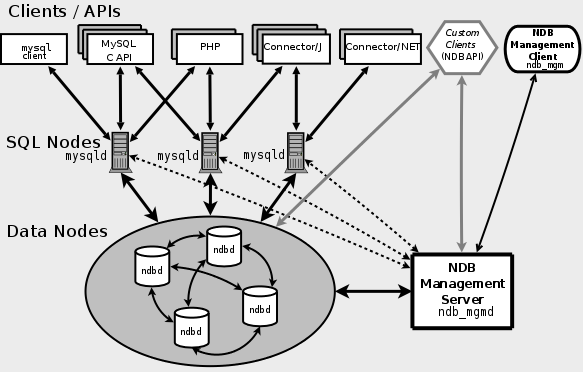
\includegraphics[width=0.75\textwidth]{image/mysql-cluster-install.png}
    \caption[ساختار خوشه‌ای پایگاه داده]
    {
      در این تصویر ساختار خوشه‌ای \lr{MySQL} نمایش داده شده است. بر اساس این
      ساختار کاربران می‌توانند پیش نیازهای سیستم را در نصب خوشه‌ای و تفاوت آن را
      با دیگر روش‌های نصب در این نرم افزار درک کند.
      از این شکل در راهنمای نصب این نرم‌افزار استفاده شده است.
    }
    \label{تصویر-ساختار-خوشه-پایگاه-داده}
  \end{figure}
  
   کاربران سیستم در اولین برخورد و مبتنی بر مستندهای این بخش است که قادر خواهند بود
   سیستم را به صورت عملی نصب کرده و به کار ببرند. لذا طراحی و نوشتن مناسب این بخش
   می‌تواند در جلب اعتماد کاربران بسیار مفید باشد. به این نکته توجه داشته باشید
   که زمانی یک کاربر به سیستم اعتماد کند آن را به کار خواهد بست و در ادامه
   تنظیم‌های پیشرفته سیستم را نیز فرا خواهد گرفت. پژوهشها نشان می‌دهد که عدم
   توانایی نصب راحت و به کار گیری یک سیستم منجر به کاهش علاقه کاربران در به
   کارگیری سیستم خواهد شد از این رو پرداختن به این بخش می‌تواند بسیار مهم باشد.

\paragraph{آزمون و خطایابی}
    تمام سیستم‌های نرم‌افزاری و سخت‌افزاری از روش‌های متفاوتی برای نمایش حالت
    درونی سیستم استفاده می‌کنند.
    واسطه‌ها گرافیکی، پیام‌های صوتی تصویری، دریچه‌های محاوره‌ای بخشی از روکردهای
    مورد استفاده در نمایش حالت درونی یک سیستم نرم‌افزاری است. سیستم‌های
    نرم‌افزاری با استفاده از همین رویکردها رویدادهای داخلی سیستم را به
    کاربران گزارش می‌کنند.

    در این بخش باید به صورت کامل به خطاهای احتمالی در فرآیند نصب یک نرم‌افزار
    پرداخته شده و راه مناسب رفع آنها به صورت کامل تشریح شود. اطلاعات موجود در
    این بخش می‌تواند کاربران را در نصب و راه‌اندازی راحت سیستم یاری کند.

    برای نمونه فرض کنید که سیستمی فیزیکی وجود دارد و در جلو آن چراغی با چهار
    رنگ قرار تعبیه شده است.
    این سیستم با استفاده از رنگهای متفاوت این چراغ‌ها حالت درونی خود را به کاربران
    سیستم گزارش می‌کند.
    از این رو در این بخش از مستند به تشریح مفهوم رنگ‌های متفاوت و روش برخورد با هر 
یک بیان می‌شود. برای نمون چراغ قرمز به معنی مناسب نبودن
    منبع تغذیه است که در این صورت باید سیستم خاموش شده و منبع تغذه آن تعمیر شود.

    تشریح روش‌های مناسب آزمون سیستم بعد از نصب نیز یکی دیگر موضوعاتی است که در
    این بخش به آن پرداخته می‌شود. اطمینان از نصب بودن و درستی حالت درونی یک
    سیستم برای استفاده عملی از آن بسیار اساسی است.

\paragraph{به روز رسانی}
    علاوبه بر نصب یک سیستم نرم‌افزاری به روز رسانی آن نیز از اهمیت زیادی
    برخوردار است. کاربران باید به صورت کامل از فرآیند به روز رسانی سیستم آگاه
    بوده و بتواند سیستم را به روز کند.

    محدودیت‌های به روز رسانی و یا توافق نامه‌های مورد نیاز در به روز رسانی
    باید در این بخش مورد بررسی قرار گیرد. کاربران بر اساس این توافق نامه
    می‌توانند در مورد استفاده یا عدم استفاده از یک بسته نرم‌افزاری تصمیم بگیرند.
    
\subsection{مبانی}

مبانی در اینجا، آن دسته از دانش‌های فنی است که نرم‌افزار مبتنی بر آنها توسعه یافته است.
برای نمونه می‌توان بسته‌های متفاوتی نام برد که بر اساس مبانی خاص ریاضی توسعه یافته‌اند
و در کاربردهای خاص مورد استفاده قرار می‌گیرند. مبانی مورد استفاده باید به صورت کامل و روشن
بیان شود تا نه تنها توسط تیم توسعه در آیند، بلکه کاربران سیستم مورد استفاده قرار گیرد.

حجم مستند مبانی ممکن است از یک صفحه تا چندین بخش قابل متغییر باشد، اما نکته‌ای که باید در نوشتن
مبانی مورد توجه قرار گیرد بیان کامل و روشن تمام مبانی مورد استفاده است. این نکته به ویژه زمانی
که نظریه‌های متفاوتی در راستای اهداف پروژه وجود دارد و تمییز بین این نظریه‌ها از اهمیت
ویژه‌ای برخوردار است، پر اهمیت می‌شود.
  
\subsection{کاربردها}
بی شک هر سیستم بر اساس اهداف از پیش تعریف شده‌ای سازمان دهی و پیاده‌سازی می‌شود. اهداف سیستم 
در بسیاری از موارد منجر به ایجاد بسیاری از محدودیت‌ها در سیستم پیاده‌سازی شده خواهد شد، از این
رو لازم است که نه تنها تمام کاربردهای نرم‌افزار بلکه محدودیت‌های آن نیز به صورت کامل بیان شود.
در این بخش تمام کاربردهای و محدودیت‌های سیستم بیان و به صورت کامل مورد بررسی قرار خواهد گرفت.
  
\subsection{پرسشهای متداول}
نمی‌توان تصور کرد که مستند ایجاد شده برای یک سیستم به صورت کامل واضح و کامل است. بسیاری از کاربران
طی استفاده از سیستم‌ها با پرسش‌های روبرو می‌شوند که به خوبی می‌تواند کاستی‌های مستندهای موجود را بیان 
می‌کند. در این برگه متداول‌ترین پرسش‌های مطرح در بین کاربران تعیین و به صورت کامل پاسخ داده می‌شود
تا به واضح‌تر شدن مستند فنی و کاربردهای نرم‌افزار بیفزاید.
  
\subsection{پیمان نامه‌ها}
مهم‌ترین قسمت یک مستند فنی، پیمان‌نامه آن است. در این قسمت از مستند به صورت کامل محدودیت‌های نرم‌افزار
ایجاد شده از نظر حقوقی بیان می‌شود که در انتخاب و به کارگیری هر سیستمی مهم است. گروه‌های متفاوت
از پیمان نامه‌های متفاوت استقبال و نرم‌افزارهای مورد نیاز خود را بر اساس همین پیمان نامه‌ها 
انتخاب می‌کنند.
  

